\subworkpkg{1.1}

%% Tasks

%% A. Search for 5 existing (or planned) similar missions and identify
%% for these missions:

%% a. the mission objectives and, if possible, the associated mission
%% requirements;

%% b. the main elements that make up the mission and their main
%% function(s);

%% c. the main performance and design characteristics of these
%% elements.

%% B. Define the mission elements with which the design process will
%% interact (e.g.: mission operations, ground system, launch system,
%% etc.).

%% C. List the main objectives to be achieved in the design process
%% (related to, e.g., payload capability, performance, structure,
%% etc.). Mention at least 10 objectives.

%% D. For each one of the identified design objectives, list the main
%% functionalities that the design must provide in order to accomplish
%% it.

%% E. List all the design parameters that are already available (e.g.,
%% from the project description provided in Section 3) and the ones
%% which still need to be identified.

%% Deliverables

%% D1.1.1. Comparative table including all the relevant information
%% collected for the reference missions identified under Task A above.

\deliverable{1.1.1}

\subsection{Similar missions}

\begin{longtable}{ll}
  \caption{Similar missions.} \\

  Mission & Launch date \\ \midrule

  Galileo & October 1989 \\

  Juno & August 2011 \\

  Jupiter Europa Orbiter (JEO) & February 2020 \\

  Jupiter Icy Moon Explorer (JUICE) & 2022 \\

  Cassini & October 1997 \\
\end{longtable}

\subsection{Mission objectives and associated requirements}

\begin{longtable}{p{.9\textwidth}}
  \caption{Similar missions' objectives and associated requirements.}
  \\

  Galileo \\* \midrule

  \begin{itemize}
  \item Study Jupiter's atmosphere, satellites, and magnetosphere by
    deploying a Jupiter orbiter and conducting various experiments.
  \item Send a probe to the surface of Jupiter to identify atmospheric
    materials and conditions that cannot be detected from outside.
  \item Venus and Earth flyby for extensive survey of the planets'
    surface and atmosphere (including imaging).
  \end{itemize}

  Requirements. Durable spacecraft and orbiter. Safe transmission of
  the data to Earth.  Strongly built probe which can survive
  penetration of the atmosphere as well as ground impact and operate
  without malfunctions. \\ \pagebreak

  Juno \\* \midrule

  \begin{itemize}
  \item Observe Jupiter's gravity and magnetic fields, atmospheric
    dynamics and composition. Thus, ultimately, investigate the
    formation and evolution of Jupiter.
  \end{itemize}

  Requirements. Durable spacecraft with maneuverability. Safe
  transmission of data to Earth. \\

  JEO \\* \midrule

  \begin{itemize}
  \item Europa's ocean. Characterize the extent of the ocean and its
    relation to the deeper interior.
  \item Europa's ice shell. Characterize the ice shell and any
    subsurface water, including their heterogeneity, and the nature of
    surface-ice-ocean exchange.
  \item Europa's chemistry. Determine global surface compositions and
    chemistry, especially as related to habitability.
  \item Europa's geology. Understand the formation of surface
    features, including sites of recent or current activity, and
    identify and characterize candidate sites for future in situ
    exploration.
  \item Jupiter system. Understand Europa in the context of the
    Jupiter system.
  \end{itemize} \\

  JUICE \\* \midrule

  \begin{itemize}
  \item Characterize the conditions that may have led to the emergence
    of habitable environments among the Jovian icy satellites, with
    special emphasis on the three ocean-bearing worlds, Ganymede,
    Europa, and Callisto.
  \end{itemize}

  Requirements. 2 flybys of Europa, 12 flybys of Callisto. Orbit
  around Ganymede. Optimal illumination conditions and high pointing
  accuracy for high-resolution imaging. Different orbits possible. A
  minimum average downlink of 1.4Gb/day. \\ \pagebreak

  Cassini \\* \midrule

  \begin{itemize}
  \item Bring the Huygens probe to Saturn's moon Titan.
  \item Study the moons Titan and Enceladus as well as the other icy
    moons.
  \end{itemize} \\
\end{longtable}

\subsection{Main mission elements and their main functions}

\begin{longtable}{p{.9\textwidth}}
  \caption{Similar missions' main elements and their main functions.}
  \\

  Galileo \\* \midrule

  \begin{itemize}
  \item Launch on a Space Shuttle. Reach the escape velocity of Earth
    and head to Jupiter.
  \item Fly past the Moon, Venus and several asteroids. Carry out
    observation and imaging.
  \item Send a probe into Jupiter's atmosphere. Identify atmospheric
    constituents and conditions.
  \item Send the orbiter into Jovian orbit. Observe the surface,
    atmosphere, and magnetosphere of Jupiter.
  \item Terminate the mission by plunging into Jupiter's
    atmosphere.
  \end{itemize} \\

  Juno \\* \midrule

  \begin{itemize}
  \item Launch on a Space Shuttle. Reach Earth escape velocity and
    head for Jupiter.
  \item Earth flyby and gravity assist.
  \item Flight to Jupiter and arrival into Jovian orbit.
  \end{itemize} \\ \pagebreak

  JEO \\* \midrule

  \begin{itemize}
  \item Launch on a Space Shuttle Atlas V 551. Reach Earth
   escape velocity and head for Jupiter.
  \item Venus and Earth flyby and gravity assist.
  \item Flight to Jupiter, and Jovian orbit insertion.
  \item Transfer to Europa orbit and Europa orbit insertion followed
    by science mapping phase.
  \item Termination of the mission. Impact the surface of Europa after
    running out of fuel.
  \end{itemize} \\

  JUICE \\* \midrule

  \begin{itemize}
  \item Launch by Ariana-5 ECA.
  \item Cruise. Interplanetary transfer from Earth to Jupiter.
  \item Jupiter tour. A transfer to Callisto, 2 Europa and 3 Callisto
    flybys, Jupiter high latitude phase, including 9 Callisto flybys,
    and finally a transfer to Ganymede.
  \item Ganymede tour, consisting of elliptical and high altitude
    circular phases, \SI{500}{km} altitude orbit and a \SI{200}{km}
    altitude orbit.
  \item End of mission.
  \end{itemize} \\

  Cassini \\* \midrule

  \begin{itemize}
  \item Launch.
  \item Jupiter flyby to provide the final push for the trajectory to
    Saturn and to study Jupiter from two different spacecraft at the
    same time.
  \item Release of the Huygens probe to Titan.
  \item Start extended mission in which different moons of Saturn are
    studied.
  \end{itemize} \\
\end{longtable}

\pagebreak
\subsection{Main mission performance and design characteristics}

\begin{longtable}{p{.9\textwidth}}
  \caption{Similar missions' main performance and design
    characteristics.} \\

  Galileo \\* \midrule

  \begin{itemize}
  \item Launch vehicle: Space Shuttle Atlantis (STS-34R).
  \item The spacecraft's propulsion module consists of twelve 10
    newton (2.25 pound-force) thrusters and a single 400 newton (90
    pound-force) engine which use monomethylhydrazine fuel and
    nitrogen-tetroxide oxidizer
  \item Spacecraft Instruments:
    \begin{itemize}
    \item Orbiter instruments:
      Imaging system.
      Near-inf\-ra\-red mapping spectrometer.
      Ultraviolet spectrometer.
      Pho\-to\-po\-la\-ri\-me\-ter-radiometer.
      Magnetometer.
      E\-ner\-ge\-tic-par\-tic\-les detector.
      Plasma detector.
      Plasma wave and heavy ion counter. Radio system
    \item Probe instruments: Atmospheric structure instrument.
      Neutral mass spectrometer. Helium abundance detector. Net flux
      radiometer. Nephelometer. Lightning and energetic particles
      experiment.
    \end{itemize}
  \item Spacecraft Power: Two radioisotope thermoelectric generators.
  \item Antenna diameter: \SI{4.8}{m}.
  \end{itemize} \\ \pagebreak

  Juno \\* \midrule

  \begin{itemize}
  \item Launch vehicle: Atlas V551
  \item Fuel mass: \SI{1280}{kg} of fuel and \SI{752}{kg} of oxidizer.
  \item Spacecraft instruments: Gravity Science Experiment.
    Magnetometer. Microwave radiometer. Particle detector. Jovian
    Infrared Auroral Mapper (JIRAM). Ultraviolet Imaging Spectrograph
    (UVS).
  \item Spacecraft power: Solar arrays. The dimensions of each solar array
    are 29.5 feet (\SI{9}{m}) by 8.7 feet (\SI{2.65}{m}).
  \item Propulsion: A dual mode propulsion subsystem. A bipropellant
    main engine supported by monopropellant reaction control system
    thrusters. The 12 reaction control system thrusters allow
    translation and rotation about three axes.
  \item Command and data handling: A RAD750 flight processor with 256
    megabytes of flash memory and 128 megabytes of DRAM local
    memory. Provides 100 Mbps total instrument throughput.
  \item Power is generated by three solar arrays of 11
    solar panels and one MAG boom.
  \end{itemize} \\ \pagebreak

  JEO \\ \midrule
  \begin{itemize}
  \item Launch Vehicle: Atlas V551.
  \item Radiation shielding to protect electronic components and
    assemblies.
  \item Telecommunications: \SI{3}{m} HGA with a 2-axis
    gimbal. \SI{25}{W} X-band and Ka-band TWTAs.
  \item Attitude control: 3-axis stabilized with reaction wheels and
    coupled thrusters.
  \item Power: \SI{540}{W} RPS (MMRTG or ASRG). Lithium ion battery
    for peak power management.
  \item Propulsion: Bipropellant, \SI{900}{N} engine.
  \item Spacecraft instruments: Laser Altimeter (LA). Radio Science
    (RS). Ice Penetrating Radar (IPR). VIS-IR Imaging Spectrometer
    (VIRIS). UV Spectrometer (UVS). Ion and Neutral Mass Spectrometer
    (INMS). Thermal Instrument (TI). Narrow Angle Camera (NAC). Wide
    Angle Camera and Medium Angle Camera (WAC+MAC). Magnetometer
    (MAG). Particle and Plasma Instrument (PPI).
  \end{itemize} \\

  JUICE \\* \midrule

  \begin{itemize}
  \item 3-axis stabilized.
  \item Solar panels: \SI{636}{W}--\SI{693}{W} (EOM).
  \item High gain antenna: \SI{3.2}{m}. Body fixed.
  \item X and Ka bands. Downlink 1.4 Gbit/day.
  \item High $\Delta V$ capability: \SI{2700}{m/s}.
  \item Radiation level: \SI{240}{krad/cm}. Al solid sphere.
  \item Dry mass at launch: \SI{1800}{kg}.
  \end{itemize} \\ \pagebreak

  Cassini \\* \midrule

  \begin{itemize}
  \item 3-axis stabilized.
  \item \SI{2150}{kg} orbiter.
  \item \SI{350}{kg} probe.
  \item \SI{3132}{kg} fuel.
  \item 3 radioisotope thermoelectric generators for
    \SI{880}{W}. \SI{670}{W} left in 2010.
  \end{itemize} \\
\end{longtable}

\subsection{Sources}

\begin{longtable}{ll}
  \caption{Sources.} \\

  Galileo & \cite{galileonasa,galileojpl} \\

  Juno & \cite{junonasa} \\

  JEO & \cite{jeonasa} \\

  JUICE & \cite{juiceesa} \\

  Cassini & \cite{cassininasa} \\
\end{longtable}

%% D1.1.2. Block diagram showing the outcomes of Task B above (hint:
%% you can put the item to be designed in the middle, and the relevant
%% mission elements around it).

\deliverable{1.1.2}

The design will have to interact with the following mission elements

\begin{figure}[h]
  \caption{Mission elements.}
  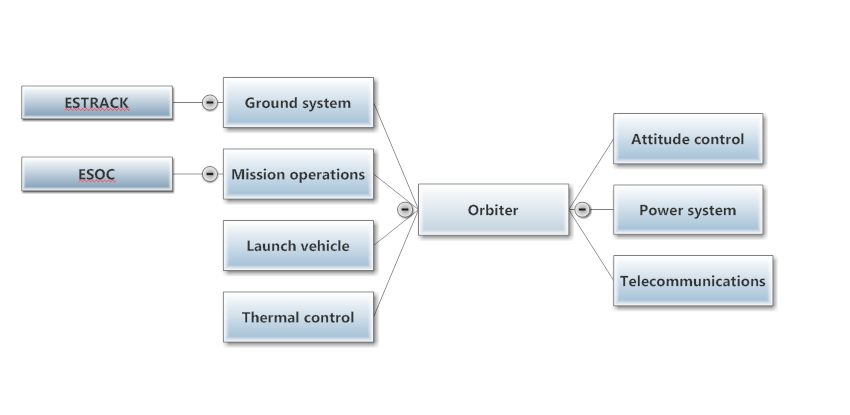
\includegraphics[width=\textwidth]{block-diagram-WP1-1B}
\end{figure}

\begin{itemize}
\item{Ground system.} The ground segment will use ESTRACK.
\item{Mission operations.} The mission operations center will be ESOC.
\item{Launch vehicle.}
\item{Thermal control.}
\item{Attitude control.}
\item{Power system.}
\item{Telecommunications.}
\item{Radiation shielding.}
\item{Propulsion systems.}
\item{S/C structures.}
\item{Orbit / trajectory}
\end{itemize}

%% D1.1.3. Numbered lists obtained from Tasks C, D and E above (note:
%% lists should be as complete as it is possible at this stage of the
%% design, and a clear justification for each listed item shall be
%% provided).

\deliverable{1.1.3}

\subsection{Mission objectives}
The following mission objectives must be met

\begin{enumerate}
\item{Payload size.} $\SI{0.7}{m} \cdot \SI{0.7}{m} \cdot \SI{0.7}{m}$
\item{Payload orientation.} Free view for camera, etc.
\item{$\Delta V$ budget.} To be determined.
\item{Power requirements.} Maximum payload power is \SI{50}{W}
\item{Payload operational temperature.} \SI{150}{K}--\SI{200}{K}
\item{Lifetime.} More than 3 years.
\item{Data storage and transfer.} To be determined.
\item{Reliability.} At least 0.9.
\item{Shielding (radioactive radiation).} To be determined.
\end{enumerate}

\subsection{Design parameters}
The already known design parameters are

\begin{enumerate}
\item{Payload mass.} \SI{80}{kg}
\item{Payload dimensions.} $\SI{0.7}{m} \cdot \SI{0.7}{m} \cdot \SI{0.7}{m}$
\item{Payload required power.} \SI{50}{W}
\item{Payload operational temperature range.} \SI{150}{K}--\SI{200}{K}
\item{Orbit.} Polar, \SI{200}{km} above Europa surface.
\item{Mission duration.} At least 3 years in Europa orbit.
\item{Launch date.} Around 2020.
\item{Total mission cost.} Less than 500 million FY2000 USD.
\item{Mission reliability.} 0.9.
\end{enumerate}
The design parameters yet to be determined include

\begin{enumerate}
\item{Radiation environment and shielding.} Radiation levels demand adequate
  shielding.
\item{$\Delta V$ budget.}
\item{Payload orientation.} Free field of view for instruments.
\item{Data storage and transfer.}
\end{enumerate}
